% Created 2020-10-15 四 21:30
% Intended LaTeX compiler: pdflatex
\documentclass[11pt]{article}
\usepackage[utf8]{inputenc}
\usepackage[T1]{fontenc}
\usepackage{graphicx}
\usepackage{grffile}
\usepackage{longtable}
\usepackage{wrapfig}
\usepackage{rotating}
\usepackage[normalem]{ulem}
\usepackage{amsmath}
\usepackage{textcomp}
\usepackage{amssymb}
\usepackage{capt-of}
\usepackage{hyperref}
\usepackage{minted}
% TIPS
% \substack{a\\b} for multiple lines text





% pdfplots will load xolor automatically without option
\usepackage[dvipsnames]{xcolor}

\usepackage{forest}
% two-line text in node by [two \\ lines]
% \begin{forest} qtree, [..] \end{forest}
\forestset{
  qtree/.style={
    baseline,
    for tree={
      parent anchor=south,
      child anchor=north,
      align=center,
      inner sep=1pt,
    }}}
%\usepackage{flexisym}
% load order of mathtools and mathabx, otherwise conflict overbrace

\usepackage{mathtools}
%\usepackage{fourier}
\usepackage{pgfplots}
\usepackage{amsthm, mathabx,  amsmath, commath}
\usepackage{amsfonts}

\usepackage{empheq}
\usepackage{tikz}
\usetikzlibrary{arrows.meta}
\usepackage[most]{tcolorbox}

\newtheorem{theorem}{Theorem}[section]
\newtheorem{definition}{Definition}[section]
\newtheorem{corollary}{Corollary}[section]
\newtheorem{example}{Example}[section]
\newtheorem{lemma}{Lemma}[section]
\newtheorem{proposition}{Proposition}[section]

\newcommand{\bl}[1] {\boldsymbol{#1}}
\newcommand{\Wt}[1] {\stackrel{\sim}{\smash{#1}\rule{0pt}{1.1ex}}}
\newcommand{\wt}[1] {\widetilde{#1}}


%For boxed texts in align, use Aboxed{}
%otherwise use boxed{}

\DeclareMathSymbol{\widehatsym}{\mathord}{largesymbols}{"62}
\newcommand\lowerwidehatsym{%
  \text{\smash{\raisebox{-1.3ex}{%
    $\widehatsym$}}}}
\newcommand\fixwidehat[1]{%
  \mathchoice
    {\accentset{\displaystyle\lowerwidehatsym}{#1}}
    {\accentset{\textstyle\lowerwidehatsym}{#1}}
    {\accentset{\scriptstyle\lowerwidehatsym}{#1}}
    {\accentset{\scriptscriptstyle\lowerwidehatsym}{#1}}
}

\usepackage{graphicx}
    
% text on arrow for xRightarrow
\makeatletter
%\newcommand{\xRightarrow}[2][]{\ext@arrow 0359\Rightarrowfill@{#1}{#2}}
\makeatother


\def \bx {\boldsymbol{x}}
\def \ba {\boldsymbol{a}}
\def \bI {\boldsymbol{I}}
\def \bt {\boldsymbol{t}}
\def \bb {\boldsymbol{b}}
\def \bA {\boldsymbol{A}}
\def \bX {\boldsymbol{X}}
\def \bu {\boldsymbol{u}}
\def \bS {\boldsymbol{S}}
\def \bZ {\boldsymbol{Z}}
\def \bz {\boldsymbol{z}}
\def \by {\boldsymbol{y}}
\def \bw {\boldsymbol{w}}
\def \bT {\boldsymbol{T}}
\def \bS {\boldsymbol{S}}
\def \bm {\boldsymbol{m}}
\def \bW {\boldsymbol{W}}
\def \bY {\boldsymbol{Y}}
\def \bH {\boldsymbol{H}}
\def \blambda {\boldsymbol{\lambda}}
\def \bPhi {\boldsymbol{\Phi}}
\def \btheta {\boldsymbol{\theta}}
\def \bmu {\boldsymbol{\mu}}
\def \bphi {\boldsymbol{\phi}}
\def \bSigma {\boldsymbol{\Sigma}}
\def \lb {\left\{}
\def \rb {\right\}}
\def \caln {\mathcal{N}}
\def \dissum {\displaystyle\Sigma}
\def \dispro {\displaystyle\prod}
\def \E {\mathbb{E}}
\def \Q {\mathbb{Q}}
\def \V {\mathbb{V}}
\def \R {\mathbb{R}}
\def \calq {\mathcal{Q}}
\def \calg {\mathcal{G}}
\def \caln {\mathcal{N}}
\def \calr {\mathcal{R}}
\def \calm {\mathcal{M}}
\def \calc {\mathcal{C}}
\def \bcup {\bigcup}

\author{M. A. Armstrong}
\date{\today}
\title{Basic Topology}
\hypersetup{
 pdfauthor={M. A. Armstrong},
 pdftitle={Basic Topology},
 pdfkeywords={},
 pdfsubject={},
 pdfcreator={Emacs 26.3 (Org mode 9.4)}, 
 pdflang={English}}
\begin{document}

\maketitle
\tableofcontents \clearpage\section{Introduction}
\label{sec:org3462b5b}
\subsection{Abstract spaces}
\label{sec:org7ec4c2e}
We ask for a set \(X\) and for each point \(x\) of \(X\) a nonempty
collection of subsets of \(X\), called neighbourhoods of \(x\). These
neighbourhoods are required to satisfy four axioms
\begin{enumerate}
\item \(x\) lies in each of its neighbourhoods
\item The intersection of two neighbourhoods of \(x\) is itself a neighbourhood
of \(x\)
\item If \(N\) is a neighbourhood of \(x\) and if \(U\) is a subset of \(X\)
which contains \(N\), then \(U\) is a neighbourhood of \(x\)
\item If \(N\) is a neighbourhood of \(x\) and if \(\mathring{N}\) denotes the set
\(\{z\in N\mid N\text{ is a neighbourhood of }z\}\), then \(\mathring{N}\) is a
neighbourhood of \(x\). (The set \(\mathring{N}\) is called the \textbf{interior} of \(N\))
\end{enumerate}


This whole structure is called a \textbf{topological space}. The assignment of a
collection of neighbourhoods satisfying axioms \((1)\to(4)\) to each point
\(x\in X\) is called a \textbf{topology} on the set \(X\).

\index{continuous}
Let \(X\) and \(Y\) be topological spaces. A function \(f:X\to Y\) is
\textbf{continuous} if for each point \(x\in X\) and each neighbourhood \(N\) of
\(f(x)\) in \(Y\) the set\(f^{-1}(N)\) is a neighbourhood of \(x\) in \(X\).
A function \(h:X\to Y\) is called a \textbf{homeomorphism} if it is one-one, onto,
continuous and has a continuous inverse. When such a function exists, \(X\)
and \(Y\) are called \textbf{homeomorphic} spaces

\begin{examplle}[]
\begin{enumerate}
\item Let \(X\) be a topological space and let \(Y\) be a subset of \(X\). We
can define a topology on \(Y\) as follows. Given a point \(y\in Y\) take
the collection of its neighbourhoods in the topological space \(X\) and
intersect each of these neighbourhood with \(Y\). The resulting sets are
the neighbourhoods of \(y\) in \(Y\). We say that \(Y\) has the \textbf{subspace topology}.
\end{enumerate}
\end{examplle}

\begin{definition}[]
A \textbf{surface} is a topological space in which each point has a neighbourhood
homeomorphic to the plane, and for which any two distinct points possess
disjoint neighbourhoods
\end{definition}

\section{Continuity}
\label{sec:org4ad711e}

\subsection{Open and closed sets}
\label{sec:orgd47a653}
Let \(X\) be a topological space and call a subset \(O\) of \(X\) \textbf{open} if
it is a neighbourhood of each of its points. The union of any collection of
open sets is open by axiom (3) and the intersection of \emph{finite} number of
open sets is open by axiom (2).


\index{neighbourhood}
Suppose we have a set \(X\) together with a nonempty collection of subsets of
\(X\), which we call open sets, such that any union of open sets is itself
open, any finite intersection of open sets is open, and both the whole set
and the empty set are open. Given a point \(x\) of \(X\), we shall call a
subset \(N\) of \(x\) a \textbf{neighbourhood of} \(x\) if we can find an open set
\(O\) s.t. \(x\in O\subseteq N\)


We claim that this definition of neighbourhood makes \(X\) into a topological
space.

Verification for axiom (4). Suppose \(N\) is a neighbourhood of \(x\) and let
\(\mathring{N}\) denote the set of points \(z\) s.t. \(N\) is a neighbourhood of
\(z\). Choose an open set \(O\) s.t. \(x\in O\subseteq N\). Now \(O\), being
open, is a neighbourhood of each of its points, so \(O\) is contained in
\(\mathring{N}\).

\begin{definition}[]
A \textbf{topology} on a set \(X\) is a nonempty collection of subsets of \(X\),
called open sets, such that any union of open sets is open, any finite
intersection of open sets is open, and both \(X\) and the empty set are open.
A set together with a topology on it is called a \textbf{topological space}
\end{definition}

The open sets of the ``usual'' topology on \(\R^n\) are characterized as
follows. A set \(U\) is open if given \(x\in U\) we can always find a
positive real number \(\epsilon\) s.t. the ball with centre \(x\) and radius
\(\epsilon\) lies entirely in \(U\).

For \textbf{discrete topology} on \(X\), every subset of \(X\) is an open set and we
call \(X\) discrete space.

A subset of a topological space is \textbf{closed} if its complement is open.

Consider the set \(A\) on \(\R^2\) whose points \(x,y\) satisfy \(x\ge0\) and
\(y>0\). This set is neither closed nor open. Take the space \(X\) whose
points are those points \((x,y)\in\R^2\) s.t. \(x\ge1\) or \(x\le-1\) and
whose topology is induced from \(\R^2\). The subsets of \(X\) consisting of
those points with positive first coordinate is both open and closed.


\index{limit point}
Let \(A\) be a subset of a topological space \(X\) and call a point \(p\) of
\(X\) a \textbf{limit point} (or accumulation point) of \(A\) if every neighbourhood
of \(p\) contains at least one point of \(A-\{p\}\)

\begin{examplle}[]
\begin{enumerate}
\item Take \(X\) to be the real line \(\R\), and let \(A\) consist of the points
\(1/n\), \(n=1,2,\dots\). Then \(A\) has exactly one limit point, namely
the origin
\item X the real line, take \(A=[0,1)\). Then each point of \(A\) is a limit
point of \(A\), and in addition \(1\) is a limit point
\item Let \(X\subseteq\R^3\) and let \(A\) consist of those points all of whose
coordinates are rational. Then every point of \(\R^3\) is a limit point of \(A\)
\item Let \(A\subseteq\R^3\) be the set of points which have integer
coordinates. Then \(A\) does not have any limit points
\item Take \(X\) to be the set of all real numebers with the so called
\textbf{finite-complement topology}. Here a set is open if its complement is
finite or all of \(X\). If we now take \(A\) to be an infinite subset of
\(X\) (say the set of all integers), then every point of \(X\) is a limit
point of \(A\). On the other hand a finite subset of \(X\) has no limit
points in this topology
\end{enumerate}
\end{examplle}

\begin{theorem}[]
A set is closed if and only if it contains all its limit points
\end{theorem}

\begin{proof}
If \(A\) is closed, its complement \(X-A\) is open. Since an open set is a
neighbourhood of each of its points, no point of \(X-A\) can be a limit point
of \(A\).

Suppose \(A\) contains all its limit point and let \(x\in X-A\). Since \(x\)
is not a limit point of \(A\), we can find a neighbourhood \(N\) of \(x\)
which does not meet \(A\). So \(N\) is inside \(X-A\), showing \(X-A\) to be
a neighbourhood of each of its points and consequently open. Therefore \(A\)
is clsoed.
\end{proof}

The union of \(A\) and all its limit points is called the \textbf{closure} of \(A\)
and is written \(\bbar{A}\)

\begin{theorem}[]
The closure of \(A\) is the smallest closed set containing \(A\), in other
words the intersection of all closed sets which contain \(A\)
\end{theorem}

\begin{proof}
For if \(x\in X-\bbar{A}\), we can find an open neighbourhood \(U\) of \(x\)
which does not contain any points of \(A\). Since an open set is a
neighbourhood of each of its points, \(U\) cannot contain any of the limit
points of \(A\). Therefore we have an open set \(U\) s.t.
\(x\in U\subseteq X-\bbar{A}\). Consequently \(X-\bbar{A}\) is a
neighbourhood of each of its points and must be open.

Now let \(B\) be a closed set which contains \(A\). Then every limit point of
\(A\) is a limit point of \(B\) and therefore must lie in \(B\) since \(B\)
is closed. This gives \(\bbar{A}\subseteq B\)
\end{proof}

\begin{corollary}[]
A set is closed if and only if it is equal to its closure
\end{corollary}

A set whose closure is the whole space is said to be \textbf{dense} in the space

The \textbf{interior} of a set, usually written \(\mathring{A}\), is the union of
all open sets contained in \(A\). A point lies in \(\mathring{A}\) if and
only if it's a neighbourhood of \(A\).

We define the \textbf{frontier} of \(A\) to be the \(\bbar{A}\cap\bbar{X-A}\).

\index{base}

Suppose we have a topology on a set \(X\), and a collection \(\beta\) of open set
s.t. every open set is a union of members of \(\beta\). Then \(\beta\) is called a
\textbf{base} for the topology and elements of \(\beta\) are called \textbf{basic open sets}.
An equivalent formulation is to ask that given a point \(x\in X\), and a
neighbourhood \(N\) of \(x\), there is always an element \(B\) of \(\beta\) s.t.
\(x\in B\subseteq N\).

\begin{theorem}[]
Let \(\beta\) be a nonempty collection of subsets of a set \(X\). If the
intersection of any finite number of members of \(\beta\) is always in \(\beta\), and
if \(\bigcup\beta=X\), then \(\beta\) is a base for a topology on \(X\)
\end{theorem}

\subsubsection{Exercise}
\label{sec:org58c3a79}
\begin{exercise}
\label{ex2.1.5}
If \(A\)is a dense subset of a space \(X\), and if \(O\) is open in \(X\),
show that \(O\subseteq\bbar{A-O}\)
\end{exercise}

\begin{proof}
Suppose \(O\not\subseteq\bbar{A\cap O}\), then there is \(x\in O\) and
\(x\not\in\bbar{A\cap O}\). Hence there is a open set \(x\in O_x\) s.t.
\begin{equation*}
\bbar{A\cap O}\cap(O_x-\{x\})=\emptyset
\end{equation*}
But as \(x\not\in\bbar{A\cap O}\), we have
\begin{equation*}
\bbar{A\cap O}\cap O_x=\emptyset
\end{equation*}
and consequently, \(A\cap O\cap O_x=\emptyset\). But then, setting \(B=O\cap
    O_x\), \(B\) is open, but \(A\cap B=\emptyset\)
\end{proof}

\begin{exercise}
\label{ex2.1.10}
Show that the frontier of a set always contains the frontier of its
interior. How does the frontier of \(A\cup B\) relate to the frontiers of
\(A\) and \(B\)
\end{exercise}

\begin{proof}
Let \((X,\tau)\) be a topological space, and let \(A\subset X\). Let
\(x\in\Fr\interior{A}\). Then
\begin{equation*}
x\in\bbar{\interior{A}}\cap\bbar{X-\interior{A}}=
\bbar{\interior{A}}\cup\bbar{(X-A)\cup(X-\interior{A})}
\end{equation*}
Now if \(x\in\bbar{\interior{A}}\) and \(x\in\bbar{X-A}\), we are done.
So suppose that \(x\in\bbar{\interior{A}}\) and
\(x\in\bbar{A-\interior{A}}\). But then
\(x\in\bbar{\interior{A}}\cup\bbar{A-\interior{A}}=\bbar{A}\).

\(\Fr(A\cup B)\subset\Fr(A)\cup\Fr(B)\)
\end{proof}

\begin{exercise}
\label{ex2.1.11}
Let \(X\) be the set of real numbers and \(\beta\) the family of all subsets of the
form \(\{x\mid a\le x<b\text{ where }a<b\}\). Prove that \(\beta\) is a base for a
topology on \(X\) and that in this topology each member of \(\beta\) is both open
and closed. Show that this topology does not have a countable base.
\end{exercise}

\begin{proof}
Suppose this topology has a countable base \(\{B_n\}_{n\in\omega}\). Define
the function \(f:\R\to\N\) as follows: for each \(x\in\R\), let \(f(x)=n\)
s.t. \(B_n\subset[x,1+x)\)

Suppose \(x<y\) and \(f(x)=f(y)\). Hence \([x,x+1)\subset[y,y+1)\), a
contradiction 
\end{proof}

\begin{exercise}
\label{ex2.1.12}
Show that if \(X\) has a countable base for its topology, then \(X\)
contains a countable dense subset. A space whose topology has a countable
base is called a \textbf{second countable} space. A space which contains a countable
dense subset is said to be \textbf{separable}.
\end{exercise}

\begin{proof}
Let \(\{B_n\}_{n\in\omega}\) be a countable base for \(\tau\).  By the Axiom of
Choice, let \(A\) be the elements of elements \(\{a_i\}_{i\in\omega}\) s.t.
\(a_i\in B_i\). The claim is that \(\bbar{A}=X\)

Let \(\calo\in\tau\). Then \(\calo=\bigcup_jB_j\). Now, as
\(A=\bigcup_ix_i\), we have \(A\cap\calo\neq\emptyset\).
\end{proof}

\subsection{Continuous functions}
\label{sec:org6f78025}
\begin{theorem}[]
\label{thm2.6}
A function from \(X\) to \(Y\) is continuous if and only if the inverse image
of each open set of \(Y\) is open in \(X\)
\end{theorem}

A continuous function is often called a \textbf{map}

\begin{theorem}[]
The composition of two maps is a map
\end{theorem}

\begin{theorem}[]
Suppose \(f:X\to Y\) is continuous, and let \(A\subseteq X\) have the
subspace topology. Then the restriction \(f|A:A\to Y\) is continuous
\end{theorem}

\begin{theorem}[]
The following are equivalent
\begin{enumerate}
\item \(f:X\to Y\) is a map
\item If \(\beta\) is a base for the topology of \(Y\), the inverse image of every
member of \(\beta\) is open in \(X\)
\item \(f(\bbar{A})\subseteq\bbar{f(A)}\) for any subset \(A\) of \(X\)
\item \(\bbar{f^{-1}(B)}\subseteq f^{-1}(\bbar{B})\) for any subset \(B\)
of \(Y\)
\item The inverse image of each closed set in \(Y\) is closed in \(X\)
\end{enumerate}
\end{theorem}

\begin{proof}
\((2)\to(3)\). \(f(A)\subseteq\bbar{f(A)}\). If \(x\in\bbar{A}-A\) and
\(f(x)\not\in f(A)\). If \(N\) is a neighbourhood of \(f(x)\) we can find a
basic open set \(B\) in \(\beta\) s.t. \(f(x)\in B\subseteq N\). \(f^{-1}(B)\) is
open and is therefore a neighbourhood of \(x\). But \(x\) is a limit point of
\(A\), which means that \(f^{-1}(B)\) must contain a point of \(A\). So
\(B\), and therefore \(N\), contains a point of \(f(A)\).

\((3)\to(4)\).
\(f(\bbar{f^{-1}(B)})\subseteq ff^{-1}(\bbar{B})\Leftrightarrow
   f(\bbar{f^{-1}(B)})\subseteq\bbar{ff^{-1}(B)}\)

\((4)\to(5)\).
\(\bbar{f^{-1}(B)}\subseteq f^{-1}(\bbar{B})=f^{-1}(B)\).
\end{proof}

\begin{examplle}[]
Let \(C\) denote the unit circle in the complex plane, taken with the
subspace topology, and give the interval \([0,1)\) the induced topology from
the real line. Define \(f:[0,1)\to C\) by \(f(x)=e^{2\pi ix}\). \(f\) is
continuous.
We can take the set of all open segments of the circle as a base for the
topology on \(C\). Now if \(S\) is such a segment and if \(S\) does not
contain the complex number 1, then \(f^{-1}(S)\) is just an open interval of
the form \((a,b)\) where \(0<a<b<1\). If \(S\) does happen to contain 1, then
\(f^{-1}(S)\) has the form \([0,a)\cup(b,1)\), where \(0<a<b<1\). This is
open in \([0,1)\) because it is the intersection of the open set
\((-1,a)\cup(b,1)\) of the real line with \([0,1)\).

However its inverse is not continuous. Take \(O\) to be the interval
\([0,1/2)\); this is open in \([0,1)\) but its image is not open in \(C\)
\end{examplle}

A \textbf{homeomorphism} \(h:X\to Y\) is a function which is continuous, one-one, and
onto, and which has continuous inverse. From Theorem \ref{thm2.6}  we see that
a set \(O\) is open iff \(h(O)\) is open. Therefore, \(h\) induces a one-one
onto correspondence between the topologies of \(X\) and \(Y\)

\begin{examplle}[]
Let \(S^n\) denote the \(n\)-dimensional sphere whose points are those of
\(\R^{n+1}\) which have distance 1 from the origin, taken with the subspace
topology. We claim that removing a single point from \(S^n\) gives a space
homeomorphic to \(\R^n\).

Which point we remove is irrelevant because we can rotate any point of
\(S^n\) into any other; for convenience we choose to remove the point
\(p=(0,\dots,0,1)\). Now the set of points of \(\R^{n+1}\), which have zero
as their final coordinate, when given the induced topology, is clearly
homeomorphic to \(\R^n\). We define a function \(h:S^n-\{p\}\to\E\), called
\textbf{stereographic projection} as follows. If \(x\in S^n-\{p\}\), then \(h(x)\) is
the point of intersection of \(\R^n\)  and the straight line determined by
\(x\) and \(p\)

   \begin{center}
      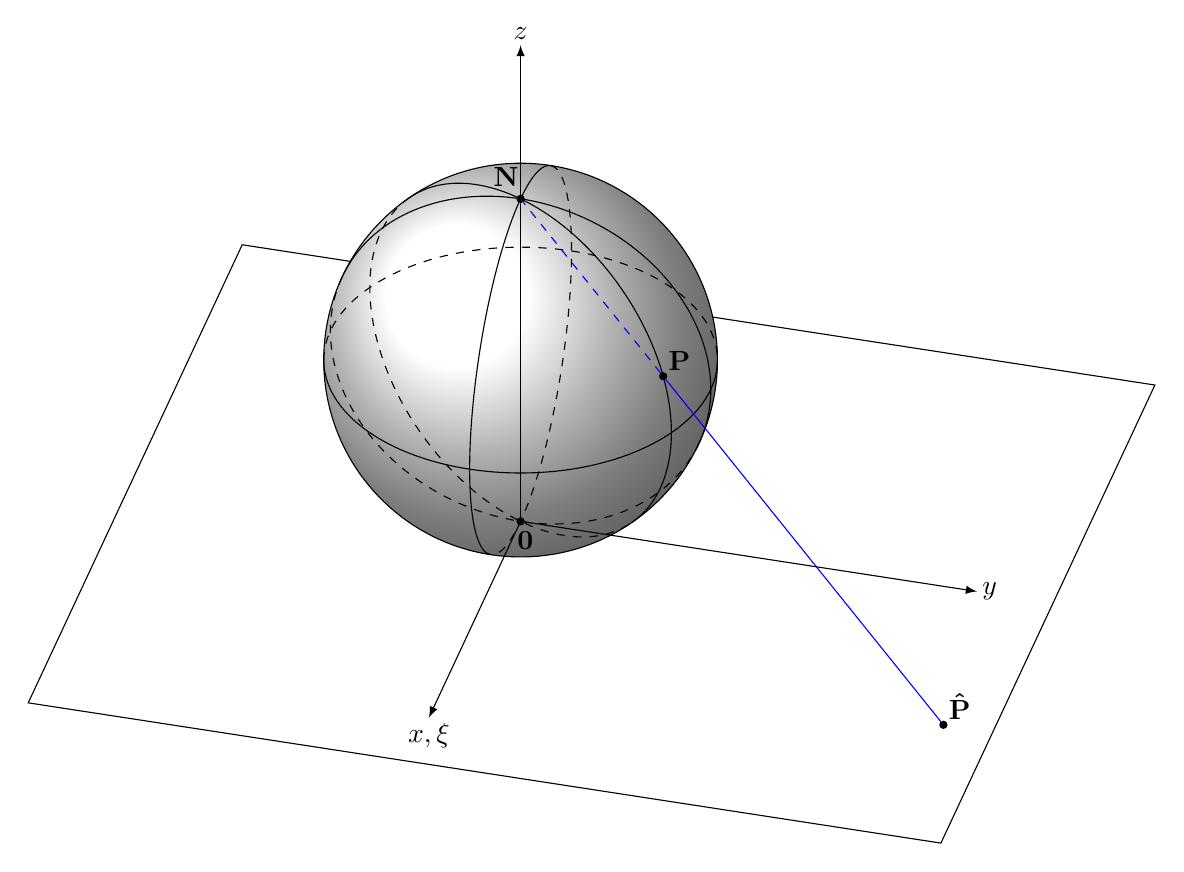
\begin{tikzpicture} % CENT
\newcommand\pgfmathsinandcos[3]{%
  \pgfmathsetmacro#1{sin(#3)}%
  \pgfmathsetmacro#2{cos(#3)}%
}
\newcommand\LongitudePlane[3][current plane]{%
  \pgfmathsinandcos\sinEl\cosEl{#2} % elevation
  \pgfmathsinandcos\sint\cost{#3} % azimuth
  \tikzset{#1/.estyle={cm={\cost,\sint*\sinEl,0,\cosEl,(0,0)}}}
}
\newcommand\LatitudePlane[3][current plane]{%
  \pgfmathsinandcos\sinEl\cosEl{#2} % elevation
  \pgfmathsinandcos\sint\cost{#3} % latitude
  \pgfmathsetmacro\yshift{\cosEl*\sint}
  \tikzset{#1/.estyle={cm={\cost,0,0,\cost*\sinEl,(0,\yshift)}}} %
}
\newcommand\DrawLongitudeCircle[2][1]{
  \LongitudePlane{\angEl}{#2}
  \tikzset{current plane/.prefix style={scale=#1}}
   % angle of "visibility"
  \pgfmathsetmacro\angVis{atan(sin(#2)*cos(\angEl)/sin(\angEl))} %
  \draw[current plane] (\angVis:1) arc (\angVis:\angVis+180:1);
  \draw[current plane,dashed] (\angVis-180:1) arc (\angVis-180:\angVis:1);
}
\newcommand\DrawLatitudeCircle[2][1]{
  \LatitudePlane{\angEl}{#2}
  \tikzset{current plane/.prefix style={scale=#1}}
  \pgfmathsetmacro\sinVis{sin(#2)/cos(#2)*sin(\angEl)/cos(\angEl)}
  % angle of "visibility"
  \pgfmathsetmacro\angVis{asin(min(1,max(\sinVis,-1)))}
  \draw[current plane] (\angVis:1) arc (\angVis:-\angVis-180:1);
  \draw[current plane,dashed] (180-\angVis:1) arc (180-\angVis:\angVis:1);
}

\tikzset{%
  >=latex, % option for nice arrows
  inner sep=0pt,%
  outer sep=2pt,%
  mark coordinate/.style={inner sep=0pt,outer sep=0pt,minimum size=3pt,
    fill=black,circle}%
}
%% some definitions

\def\R{2.5} % sphere radius
\def\angEl{35} % elevation angle
\def\angAz{-105} % azimuth angle
\def\angPhi{-40} % longitude of point P
\def\angBeta{19} % latitude of point P

%% working planes

\pgfmathsetmacro\H{\R*cos(\angEl)} % distance to north pole
\tikzset{xyplane/.estyle={cm={cos(\angAz),sin(\angAz)*sin(\angEl),-sin(\angAz),
                              cos(\angAz)*sin(\angEl),(0,-\H)}}}
\LongitudePlane[xzplane]{\angEl}{\angAz}
\LongitudePlane[pzplane]{\angEl}{\angPhi}
\LatitudePlane[equator]{\angEl}{0}

%% draw xyplane and sphere

\draw[xyplane] (-2*\R,-2*\R) rectangle (2.2*\R,2.8*\R);
\fill[ball color=white] (0,0) circle (\R); % 3D lighting effect
\draw (0,0) circle (\R);

%% characteristic points

\coordinate (O) at (0,0);
\coordinate[mark coordinate] (N) at (0,\H);
\coordinate[mark coordinate] (S) at (0,-\H);
\path[pzplane] (\angBeta:\R) coordinate[mark coordinate] (P);
\path[pzplane] (\R,0) coordinate (PE);
\path[xzplane] (\R,0) coordinate (XE);
\path (PE) ++(0,-\H) coordinate (Paux); % to aid Phat calculation
\coordinate[mark coordinate] (Phat) at (intersection cs: first line={(N)--(P)},
                                        second line={(S)--(Paux)});

%% draw meridians and latitude circles

\DrawLatitudeCircle[\R]{0} % equator
\DrawLongitudeCircle[\R]{\angAz} % xzplane
\DrawLongitudeCircle[\R]{\angAz+90} % yzplane
\DrawLongitudeCircle[\R]{\angPhi} % pzplane

%% draw xyz coordinate system

\draw[xyplane,<->] (1.8*\R,0) node[below] {$x,\xi$} -- (0,0) -- (0,2.4*\R)
    node[right] {$y$};
\draw[->] (0,-\H) -- (0,1.6*\R) node[above] {$z$};

%% draw lines and put labels

\draw[blue,dashed] (P) -- (N) +(0.3ex,0.6ex) node[above left,black] {$\mathbf{N}$};
\draw[blue] (P) -- (Phat) node[above right,black] {$\mathbf{\hat{P}}$};
\path (S) +(0.4ex,-0.4ex) node[below] {$\mathbf{0}$};
\draw (P) node[above right] {$\mathbf{P}$};
\end{tikzpicture}
   \end{center}
\end{examplle}

By a \textbf{disc} we mean any space homeomorphic to the closed unit disc \(D\) in
\(\R^2\). \(C\) stands for the unit circle. If \(A\) is a disc, and if
\(h:A\to D\) is a homeomorphism, then \(h^{-1}(C)\) is called the \textbf{boundary} of
\(A\) and is written \(\partial A\).

\begin{lemma}[]
\label{lemma2.10}
Any homeomorphism from the boundary of a disc to itself can be extended to a
homeomorphism of the whole disc
\end{lemma}

\begin{proof}
Let \(A\) be a disc and choose a homeomorphism \(h:A\to D\). Given a
homeomorphism \(g:\partial A\to\partial A\), we can easily extend \(hgh^{-1}:C\to
   C\) to a homeomorphism of all of \(D\)as follows. Send 0 to 0, and if \(x\in
   D-\{0\}\) send \(x\) to the point \(\norm{x}hgh^{-1}(x/\norm{x})\). In other
words extend conically
\end{proof}

\begin{lemma}[]
Let \(A\) and \(B\) be discs which intersect along their boundaries in an
arc. Then \(A\cup B\) is a disc.
\end{lemma}

\begin{proof}
Let \(\gamma\) denote the arc \(A\cap B\), and use \(\alpha\), \(\beta\) for the complementary arcs in
the boundaries of \(A\) and \(B\). We construct a homeomorphism from \(A\cup
   B\) to \(D\) with the aid of lemma \ref{lemma2.10}

The \(y\) axis in the plain divides up \(D\) as the union of two discs
\(D_1\) and \(D_2\). We label the three arcs which together make up the
boundaries of \(D_1\) and \(D_2\) as \(\alpha'\), \(\beta'\) and \(\gamma'\).
Both \(\alpha\) and \(\alpha'\) are homeomorphic to the clsoed unit interval
\([0,1]\), so we can find a homeomorphism from \(\alpha\) to \(\alpha'\). We first
extend this over \(\gamma\), to give a homeomorphism from \(\alpha\cup\gamma\) to
\(\alpha'\cup\gamma'\); then over \(A\) to give a homeomorphism from \(A\) to
\(D_1\), which take \(\gamma\) to \(\gamma'\), using lemma \ref{lemma2.10}.
\end{proof}


\subsubsection{Exercise}
\label{sec:orgd3d4e2b}
\begin{exercise}
\label{ex2.13}
If \(f:\R\to\R\) is a map, show that the set of points which are left fixed
by \(f\) is a closed subset of \(\R\). If \(g\) is a continuous real-valued
function on \(X\) show that the set \(\{x\mid g(x)=0\}\) is closed
\end{exercise}

\begin{proof}
Define \(f_0(x)=f(x)-x\)
\end{proof}

\begin{exercise}
\label{ex2.25}
Let \(f:\R\to\R\) be a map and define its graph \(\Gamma_f:\R\to\R^2\) by
\(\Gamma_f(x)=(x,f(x))\). Show that \(\Gamma_f\) is continuous and that its
image (taken with the topology induced from \(\R^2\)) is homeomorphic to \(\R\)
\end{exercise}

\begin{proof}
The function \(p_1:\im\Gamma_f\to\E\) defined by \((x,f(x)\mapsto x)\) is
the desired homeomorphism
\end{proof}

\begin{exercise}
\label{ex2.16}
What topology must \(X\) have if every real-valued function defined on \(X\)
is continuous
\end{exercise}

\begin{proof}
Discrete topology. It suffices to show points in \(X\) are open

Fix \(x\in X\) and define \(f:X\to\R\) by
\begin{equation*}
f(x)=
\begin{cases}
f(x)=0\\
f(y)=1&y\neq x
\end{cases}
 \end{equation*}
Then \(f^{-1}((-0.5,0.5))=\{x\}\)
\end{proof}

\begin{exercise}
An \textbf{open map} is one which sends open sets to open sets: a \textbf{closed map} takes
closed sets to closed sets. Which of the following maps are open or closed
\begin{enumerate}
\item The exponential map \(x\mapsto e^{ix}\) from the real line to the circle
\item The folding map \(f:\R^2\to\R^2\) given by \((x,y)\mapsto(x,\abs{y})\)
\item The map which winds the plane three times on itself given in terms of
complex numbers, by \(z\mapsto z^3\)
\end{enumerate}
\end{exercise}

\begin{proof}
\begin{enumerate}
\item 

\item not open. closed.
\item open. closed
\end{enumerate}
\end{proof}
\subsection{A space-filling curve}
\label{sec:org110cab6}
\subsection{The Tietze extension theorem}
\label{sec:org2506b0e}
Let \(X\) be a topological space and \(A\) a subspace of \(X\). Given a
real-valued continuous function defined on \(A\), it is natural to ask
whether or not we can always extend it to all of \(X\).

\begin{definition}[]
A \textbf{metric} or \textbf{distance function} on a set \(X\) is a real-valued function \(d\)
defined on the cartesian product \(X\times X\) s.t. for all \(x,y,z\in X\)
\begin{enumerate}
\item \(d(x,y)\ge0\) with equality iff \(x=y\)
\item \(d(x,y)=d(y,x)\)
\item \(d(x,y)+d(y,z)\ge d(x,z)\)
\end{enumerate}


A set together with a metric on it is called a \textbf{metric space}
\end{definition}

A metric on a set gives rise to a topology on the set as follows. Let \(d\)
be a metric on the set \(X\). Given \(x\in X\), the set \(\{y\in X\mid
   d(x,y)\}\le\epsilon\) is called the \textbf{ball of radius} \(\epsilon\), or
\(\epsilon\)-ball, centered at the point \(x\), and is denoted by \(B(x,\epsilon)\).
We define a subset \(O\) of \(X\) to be \textbf{open} if given \(x\in O\) we can find
a positive real number \(\epsilon\) s.t. \(B(x,\epsilon)\subset O\).

Different metrics on a set may give the same topology. For example, we can
make the underlying set of points of euclidean \(n\)-space into a metric
space in three different ways as follows. Write
\(\bx=(x_1,\dots,x_n)\in\R^n\), define:
\begin{enumerate}
\item \(d_1(\bx,\by)=\sqrt{(x_1-y_1)^2+\dots+(x_n-y_n)^2}\)
\item \(d_2(\bx,\by)=\max_{1\le i\le n}\abs{x_i-y_i}\)
\item \(d_3(\bx,\by)=\abs{x_1-y_1}+\dots+\abs{x_n-y_n}\)
\end{enumerate}


Following shows the ball of radius 1, centered at the origin for each of
these three metrics when \(n=2\).

\begin{center}
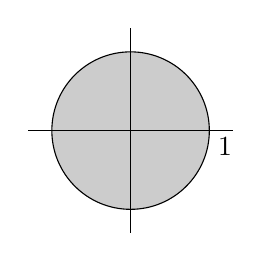
\begin{tikzpicture}
\draw[fill=black!20,draw=Black] (0,0) circle [radius=1cm];
   \draw (-1.3,0) -- (1.3,0);
\draw (0,-1.3) -- (0,1.3);
\node at (1.2,-0.2) {1};
\end{tikzpicture}
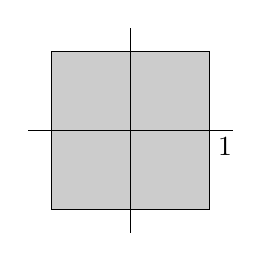
\begin{tikzpicture}
\draw[fill=black!20] (-1,-1) rectangle (1,1);
\draw (-1.3,0) -- (1.3,0);
\draw (0,-1.3) -- (0,1.3);
\node at (1.2,-0.2) {1};
\end{tikzpicture}
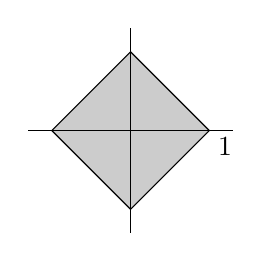
\begin{tikzpicture}
\draw[fill=black!20] (-1,0) -- (0,1) -- (1,0) -- (0,-1) -- (-1,0);
\draw (-1.3,0) -- (1.3,0);
\draw (0,-1.3) -- (0,1.3);
\node at (1.2,-0.2) {1};
\end{tikzpicture}
\end{center}

To see that \(d_1\) and \(d_2\) give rise to the same topology, we note that
inside any disc we can find a square, and conversely inside a square we can
find a disc.

Given two distinct points in a metric space, we can always find disjoint open
sets containing them. For if \(d(x,y)=\delta>0\), set \(U=\{z\in X\mid
   d(x,z)<\delta/2\}\) and \(V=\{z\in X\mid d(y,z)\le\delta/2\}\). Then both
\(U\) and \(V\) are open sets. The set \(U\) is usually called the \textbf{open ball}
with center \(x\) and radius \(\delta/2\). A topological space with the
property that two distinct points can always be surrounded by disjoint open
sets is called a \textbf{Hausdorff space}.

If \(d\) is a metric on \(X\) and if \(A\) is a subset of \(X\), the distance
\(d(x,A)\) of the point \(x\) from \(A\) is defined to be the infimum of the
numbers \(d(x,a)\) where \(a\in A\)

\begin{lemma}[]
The real-valued function on \(X\) defined by \(x\mapsto d(x,A)\) is continuous
\end{lemma}

\begin{proof}
Let \(x\in X\) and let \(N\) be a neighbourhood of \(d(x,A)\) on the real
line. Choose \(\epsilon>0\) small enough so that the interval
\((d(x,A)-\epsilon,d(x,A)+\epsilon)\) lies inside \(N\). Let \(U\) denote the
open ball centered \(x\), radius \(\epsilon/2\), \(z\in U\), and choose a point \(a\in
   A\) s.t.
\(d(x,a)<d(x,A)+\epsilon/2\). If \(z\in U\) we have
\begin{equation*}
d(z,A)\le d(z,a)\le d(z,x)+d(x,a)<d(x,A)+\epsilon
\end{equation*}
By reversing the roles of \(x\) and \(z\), we also have
\(d(x,A)<d(z,A)+\epsilon\). Therefore \(U\) is mapped inside
\((d(x,A)-\epsilon,d(x,A)+\epsilon)\) and hence inside \(N\), by our
function, showing that the inverse image of \(N\) is a neighbourhood of \(x\)
in \(X\) as required.
\end{proof}

\begin{lemma}[]
\label{lemma2.14}
If \(A,B\) are disjoint closed subsets of a metric space \(X\), there is a
continuous real-valued function on \(X\) which takes the value 1 on points of
\(A\), -1 on points of \(B\), and values strictly between \(\pm1\) on points
of \(X-(A\cup B)\)
\end{lemma}

\begin{proof}
Since \(A\) and \(B\) are both closed and are disjoint, the expression
\(d(x,A)+d(x,B)\) can never be zero by Exercise \ref{ex2.4.27}. Therefore we
can define a real-valued function \(f\) on \(X\) by
\begin{equation*}
f(x)=\frac{d(x,B)-d(x,A)}{d(x,B)+d(x,A)}
\end{equation*}
\end{proof}

\begin{lemma}[]
If \(A\)  is closed in \(Y\) and \(Y\) is closed in \(X\), then \(A\) is
closed in \(X\)
\end{lemma}

\begin{proof}
\(Y-A=B\cap Y\) and \(Y-A\subset B\). \(X-Y\cup B\) is open and \(X-Y\cup B=X-A\)
\end{proof}

\begin{definition}[]
For each \(n\in\N\), let \(f_n:A\to\R\) for \(A\subset\R\). The sequence
\((f_n)\) \textbf{converges pointwise on} \(A\) to a function \(f:A\to\R\) if for all
\(x\in A\) the sequence of real numbers \(f_n(x)\) converges to \(f(x)\)
\end{definition}

\begin{definition}[]
Let \(f_n\) be a sequence of functions defined on \(A\subset\R\). We say that
\((f_n)\) \textbf{converges uniformly on} \(A\) to a limit function \(f\) on \(A\) if
for every \(\epsilon>0\) there exists an \(N\in\N\) s.t.
\(\abs{f_n(x)-f(x)}<\epsilon\) for all \(x\in A\) whenever \(n\ge N\)
\end{definition}

\begin{definition}[]
A sequence \(\{a_n\}\) of real numbers is called a \textbf{Cauchy sequence} if for
every \(\epsilon>0\) there exists an \(N\) s.t. \(\abs{a_n-a_m}<\epsilon\) whenever
\(n,m\ge N\).
\end{definition}


\begin{theorem}[Cauchy criterion for uniform convergence]
A sequence of functions \((f_n)\) defined on \(A\subset\R\) converges
uniformly on \(A\) iff for every \(\epsilon>0\) there exists an \(N\in\N\) s.t.
\begin{equation*}
\abs{f_n(x)-f_m(x)}<\epsilon
\end{equation*}
for all \(n,m\ge N\) and for all \(x\in A\)
\end{theorem}

\begin{proof}
Suppose \(f_n\) converges uniformly to \(f\) on \(A\). Then for \(\epsilon>0\) there
exists \(N\in\N\) s.t. \(\abs{f_n(x)-f(x)}<\epsilon/2\) for all \(n\ge N\)
and all \(x\in A\)

Then for \(n,m\ge N\) and any \(x\in A\) we have
\begin{align*}
\abs{f_n(x)-f_m(x)}&=\abs{f_n(x)-f(x)+f(x)-f_m(x)}\\
&\le\abs{f_n(x)-f(x)}+\abs{f_m(x)-f(x)}\\
&<\epsilon/2+\epsilon/2\\
&=\epsilon
\end{align*}

Now suppose that for all \(\epsilon>0\) there exists \(N\in\N\) s.t.
\(\abs{f_n(x)-f_m(x)}<\epsilon\) for all \(n,m\ge M\) and all \(x\in A\)

Then for each \(x\in A\), the sequence \((f_n(x))\) is a Cauchy sequence of
real numbers, and therefore it converges to a real number, call it \(f(x)\)
(Check \href{https://proofwiki.org/wiki/Cauchy\_Sequence\_Converges\_on\_Real\_Number\_Line}{Proof}).

We have found a function \(f:A\to\R\) which is the pointwise limit of \(f_n\)

By the Algebraic Limit and Order Limit Theorem we have for all \(n\ge N\) and
all \(x\in A\) that
\begin{equation*}
\abs{f_n(x)-f(x)}=\lim_{m\to\infty}\abs{f_n(x)-f_m(x)}\le\epsilon
\end{equation*}
which says that \(f_n\) converges uniformly to \(f\) on \(A\)
\end{proof}

\begin{theorem}[Continuous limit theorem]
Let \((f_n)\) be a sequence of functions defined on \(A\subseteq\R\) that
converges uniformly on \(A\) to \(f\). If each \(f_n\) is continuous at
\(c\in A\), then \(f\) is continuous at \(c\) too
\end{theorem}

\begin{proof}
Fix \(x\in A\) and for \(\epsilon>0\) choose \(N\in\N\) s.t. for all \(x\in A\) we
have
\begin{equation*}
\abs{f_N(x)-f(x)}<\frac{\epsilon}{3}
\end{equation*}
By the continuity of \(f_N\) at \(c\) there exists \(\delta>0\) s.t. whenever
\(\abs{x-c}<\delta\) we have
\begin{equation*}
\abs{f_N(x)-f_N(c)}<\frac{\epsilon}{3}
\end{equation*}
Thus
\begin{equation*}
\abs{f(x)-f(c)}\le\abs{f(x)-f_N(x)}+\abs{f_N(x)-f_N(c)}+\abs{f_N(c)-f(c)}<\epsilon
\end{equation*}
\end{proof}



\begin{theorem}[Tietze extension theorem]
Any real-valued continuous function defined on a closed subset of a metric
space can be extended over the whole space
\end{theorem}

\begin{proof}
Let \(X\) be a metric space, \(C\) a closed subset, and \(f:C\to\R\) a map.
To begin with we shall assume that \(f\) is bounded; say \(\abs{f(x)}\le M\)
for all \(x\in C\)

Let \(A_1=\{x\mid f(x)\ge M/3\}\), \(B_1=\{x\mid f(x)\le -M/3\}\). \(A\) and
\(B\) are disjoint and are both closed in \(X\). Since \(A_1\) is the inverse
image of the closed subset \([M/3,+\infty)\) of \(\R\). \(A_1\) is closed in
\(C\), and \(C\) is closed in \(X\). Hence \(A_1\) is closed in \(X\). By
Lemma \ref{lemma2.14}, we can find a map \(g_1:X\to[-M/3,M/3]\) which takes the
value \(M/3\) on \(A_1\), \(-M/3\) on \(B_1\), and which takes values in
\((-M/3,M/3)\) on \(X-(A_1\cup B_1)\). Notice that \(\abs{f(x)-g_1(x)}\le
   2M/3\) on \(C\)

Now consider the function \(f(x)-g_1(x)\) and let \(A_2\) consists of those
points of \(C\) for which \(f(x)-g_1(x)\ge2M/9\) and \(B_2\) those points for
which \(f(x)-g_1(x)\le-2M/9\). By Lemma \ref{lemma2.14} we have a map
\(g_2:X\to[-2M/9,2M/9]\) which takes the value \(2M/9\) on \(A_2\), \(-2M/9\)
on \(B_2\). \(\abs{f(x)-g_1(x)-g_2(x)}<4M/9\) on \(C\)

By repeating this process we can construct a sequence of maps
\(g_n:X\to[-2^{n-1}M/3^n,x^{n-1}M/3^n]\) which satisfy
\begin{enumerate}
\item \(\abs{f(x)-g_1(x)-\dots-g_n(x)}\le 2^nM/3^n\) on \(C\) and
\item \(\abs{g_n(x)}<2^{n-1}M/3^n\) on \(X-C\)
\end{enumerate}


The series \(\sum_{n=1}^\infty g_n(x)\) converges uniformly on \(X\) by the
Weierstrass M-test, so it has a well-defined sum \(g(x)\) which is
continuous. Also \(f\) and \(g\) agree on \(C\) by (1). Therefore \(g\)
extends \(f\) to all of \(X\). We note, for use in the unbounded case
\(\abs{g(x)}\) is bounded by \(M\) because
\begin{equation*}
\abs{g(x)}=\sum_{n=1}^\infty\abs{g_n(x)}\le M\sum_{n=1}^\infty
x^{n-1}/c^n=M
\end{equation*}
and \(\abs{g(x)}\) is strictly less than \(M\) on \(X-C\) by (2)


If \(g\) is not bounded, choose a homeomorphism \(h\) from the real line to the
interval \((-1,1)\) and consider the composition \(h\circ f\). This is
bounded and we can extend it to a continuous real-valued function
\end{proof}

\subsubsection{Exercise}
\label{sec:org29e8573}
\begin{exercise}
\label{ex2.4.27}
Show \(d(x,A)=0\) iff \(x\) is a point of \(\bbar{A}\)
\end{exercise}

\begin{proof}
Suppose that \(d(x,A)=0=\inf_{a\in A}d(x,a)\). Then for every \(\epsilon>0\), there
exists \(a\in A\) s.t.
\begin{equation*}
\abs{d(x,a)-0}=d(x,a)<\epsilon
\end{equation*}
Now let \(\calo\) be an open subset of \(X\), \(x\in\calo\). Choose \(a\in
    A\) s.t. \(d(x,a)<\epsilon\). Then \(a\in\calo\) and \(\calo\cap
    A\neq\emptyset\). Thus \(x\in\bbar{A}\)

Suppose \(x\in\bbar{A}\). For \(n\in\N\), let \(B_n=\{y\mid d(x,y)<1/n\}\).
Then \(B_n\) is open, so \(B_n\cap A\neq\emptyset\). Let \(a_n\in B_n\cap
    A\). Then \(d(x,a_n)<1/n\) thus \(\inf_{a\in A}d(x,a)<1/n\) for every \(n\).
Thus \(\inf_{a\in A}d(x,a)=0\)
\end{proof}

\section{Compactness and Connectedness}
\label{sec:orgeb2fe19}

\subsection{Closed bounded subsets of \(\R^n\)}
\label{sec:org522131c}
Let \(X\) be a topological space and let \(\calf\) be a family of open
subsets of \(X\) whose union is all of \(X\). Such a family will be called an
\textbf{open cover} of \(X\). If \(\calf'\) is a subfamily of \(\calf\) and if
\(\bigcup\calf'=X\), then \(\calf'\) is called a \textbf{subcover} of \(\calf\).

\begin{theorem}[]
\label{thm3.1}
A subset \(X\) of \(\R^n\) is closed and bounded iff every open cover of
\(X\) (with the induced topology) has a finite subcover
\end{theorem}

\index{compact}
\begin{definition}[]
A topological space \(X\) is \textbf{compact} if every open cover of \(X\) has a
finite subcover
\end{definition}

With this terminology, theorem \ref{thm3.1} can be restated as follows.
\emph{The closed bounded subsets of a euclidean space are precisely those subsets}
\emph{which (when given the induced topology) are compact}

\subsection{The Heine-Borel theorem}
\label{sec:org2df4647}
\begin{theorem}[The Heine-Borel theorem]
\label{thm3.3}
A closed interval of the real line is compact
\end{theorem}

\begin{proof}['Creeping along' proof]
Let \([a,b]\) be a closed interval of the real line, with the induced
topology, and let \(\calf\) be an open cover of \([a,b]\). We define a subset
\(X\) of \([a,b]\) by
\begin{equation*}
X=\{x\in[a,b]\mid[a,x]\text{ is contained in the union of a finite subfamily of }\calf\}
\end{equation*}
Then \(X\) is nonempty (\(a\in X\)) and is bounded above (by \(b\)). So \(X\)
has a supremum, say \(s\). We claim that \(s\in X\) and that \(s=b\). For let
\(O\) be the member of \(\calf\) which contains \(s\). Since \(O\) is open we
can choose \(\epsilon>0\) small enough that \((s-\epsilon,s]\subseteq O\), and if
\(s\) is less than \(b\) we can assume \((s-\epsilon,s+\epsilon)\subseteq
   O\). Now \(s\) is the \emph{least} upper bound of \(X\), consequently there are
points of \(X\) arbitrarily closed to \(s\). Also, \(X\) has the property
that if \(x\in X\) and if \(a\le y\le x\) then \(y\in X\). Therefore we may
assume \(s-\epsilon/2\in X\). By the definition of \(X\), the interval
\([a,s-\epsilon/2]\) is contained in the union of some finite subfamily
\(\calf'\) of \(\calf\). Adding \(O\) to \(\calf'\) we obtain a finite
collection of members of \(\calf\) whose union certainly contains \([a,s]\).
Therefore \(s\in X\). If \(s\) is less than \(b\) then \(\bigcup\calf'\cup
   O\) contains \([a,s+\epsilon/2]\) contradicting the fact that \(s\) is an
upper bound for \(X\).
\end{proof}

\begin{proof}['subdivision' proof]
Suppose that theorem \ref{thm3.3}  is false. Let \(\calf\) be an open cover of
\([a,b]\) which does not contain a finite subcover. Set \(I_1=[a,b]\).
Subdivide \([a,b]\) into two closed subintervals of equal length
\([a,(a+b)/2]\), \([a,b]/2,b\). At least one of these have the property that
it is not contained in the union of any finite subfamily of \(\calf\). Select
one of them and call it \(I_2\).  Continuing in this way we obtain a nested
sequence of closed intervals
\begin{equation*}
I_1\supseteq I_2\supseteq I_3\supseteq\dots
\end{equation*}
whose lengths tend to zero.

We claim that \(\displaystyle\bigcap_{n=1}^\infty I_n\) consists of precisely
one point. In our first proof of theorem \ref{thm3.3}, we used the so-called
completeness property of the real numbers (a nonempty set of real numbers
which is bounded above has a least upper bound). We let \(x_n\) denote the
left-hand end point of the interval \(I_n\) and we consider the sequence
\(\{x_n\}\). This sequence is monotonic increasing and bounded. Therefore if
\(p\) denotes the supremum of the \(x_n\) we know that \(\{x_n\}\) converges
to \(p\). It's now elementary to check that \(p\in I_n\) for all \(n\). Also,
since the lengths of the \(I_n\) tend to zero as \(n\) tend to infinity, it
should be clear that \(\bigwedge_{n=1}^\infty I_n\) cannot contain more than
one point. Therefore \(\bigwedge_{n=1}^\infty I_n=\{p\}\)

Now \(p\) belongs to \([a,b]\) and so lies in some open set \(O\) of
\(\calf\). We choose \(\epsilon>0\) small enough that
\((p-\epsilon,p+\epsilon)\cap[a,b]\subseteq O\), and we choose a positive
integer \(n\) large enough that length \((I_n)<\epsilon\). Since \(p\in
   I_n\), we see that \(I_n\) is completely contained in \(O\). But \(I_n\) was
selected so that it did not lie in the union of any finite subfamily of
\(\calf\), and here we have \(I_n\) inside a single member of \(\calf\).
\end{proof}

Suppose \(f:[a,b]\to\R\) is continuous. Given \(x\in[a,b]\) we can find a
neighbourhood \(O(x)\) of \(x\) in \([a,b]\) s.t. \(\abs{f(x')-f(x)}<1\) for
all points \(x'\in O(x)\). The family of all such \(O(x)\) forms an open
cover of \([a,b]\). Therefore by the Heine-Borel theorem we can find a finite
subfamily, say \(O(x_1),\dots,O(x_k)\) s.t. \(O(x_1)\cup\dots\cup
   O(x_k)=[a,b]\). Now if \(x\in O(x_i)\) then \(\abs{f(x)}\le\abs{f(x_i)}+1\).
So for any point \(x\in[a,b]\) we have
\begin{equation*}
\abs{f(x)}\le\max\{\abs{f(x_1)},\dots,\abs{f(x_k)}\}+1
\end{equation*}


\subsubsection{Exercise}
\label{sec:orgd94122a}
\begin{exercise}
Find an open cover of \(\R\) which does not contain a finite subcover. Do
the same for \([0,1)\) and \((0,1]\)
\end{exercise}
\begin{proof}
\(I_n=[0,1-\frac{1}{n}]\). \(I_n=(\frac{1}{n},1-\frac{1}{n})\)
\end{proof}

\begin{exercise}
Let \(S\supseteq S_1\supseteq S_2\supseteq\dots\) be a nested sequence of
squares in the plane whose diameters tend to zero as we proceed along the
sequence. Prove that the intersection of all these squares consists of
exactly one point.
\end{exercise}

\begin{proof}
We have \(\{x_n\}\) and \(\{y_n\}\).
\end{proof}

\begin{exercise}
Use the Heine-Borel theorem to show that an infinite subset of a closed
interval must have a limit point
\end{exercise}

\begin{proof}
Let \(I\) be a closed interval. Let \(A\subseteq I\) be an infinite subset.
Suppose \(A\) does not have any limit points. Then for each \(x\in I\) there
is an open set \(U_x\subseteq I\) s.t. \(x\in U_x\) and \(U_x\cap
    A-\{x\}=\emptyset\). \(\{U_x\}\) is an open cover of \(I\), by the
Heine-Borel theorem there is a finite subcover
\(\{U_{x_1},\dots,U_{x_n}\}\).  It must be that \(A\subseteq
    U_{x_1}\cup\dots\cup U_{x_n}\). But the only element of each \(U_x\) that is
in \(A\) is \(x\). Thus \(U_{x_1}\cup\dots\cup U_{x_n}=\{x_1,\dots,x_n\}\) a
finite set. Thus \(A\) must be finite.
\end{proof}

\subsection{Properties of compact spaces}
\label{sec:org311d403}
\begin{theorem}[]
\label{thm3.4}
The continuous image of a compact space is compact
\end{theorem}

\begin{proof}
If \(f:X\to Y\) is an onto continuous function, and if \(X\) is compact, then
we must show \(Y\) compact. Let \(\calf\) be an open cover of \(Y\). If
\(O\in\calf\) then \(f^{-1}(O)\) is an open subset of \(X\) by the continuity
of \(f\), and so the family
\begin{equation*}
\calg=\{f^{-1}(O)\mid O\in\calf\}
\end{equation*}
is an open cover of \(X\). Since \(X\) is compact, \(\calg\) contains a
finite subcover, say \(X=f^{-1}(O_1)\cup\dots\cup f^{-1}(O_k)\). Now \(f\) is
an onto function, therefore \(f(f^{-1}(O_i))=O_i\), and we have
\(Y=O_1\cup\dots\cup O_k\).
\end{proof}

A subset of \(C\) of a topological space \(X\) is called a \textbf{compact subset of
\(X\)} if \(C\) with the induced topology from \(X\) is a compact space. \(C\)
is a compact subset of \(X\) iff every family of open subsets of \(X\) whose
union contains \(C\) has a finite subfamily whose union also contains \(C\)

\begin{theorem}[]
\label{thm3.5}
A closed subset of a compact space is compact
\end{theorem}

\begin{proof}
Let \(X\) be a compact space, \(C\) a closed subset of \(X\), and \(\calf\) a
family of open subsets of \(X\) s.t. \(C\subseteq\bigcup\calf\). If we add
the open set \(X-C\) to \(\calf\) we obtain an open cover of \(X\). Therefore
we can find \(O_1,\dots,O_k\in\calf\) s.t. \(O_1\cup\dots\cup
   O_k\cup(X-C)=X\). This gives \(C\subseteq O_1\cup\dots\cup O_k\)
\end{proof}

\begin{theorem}[]
\label{thm3.6}
If \(A\) is a compact subset of a Hausdorff space \(X\), and if \(x\in X-A\),
then there exist disjoint neighbourhoods of \(x\) and \(A\). Therefore a
compact subset of a Hausdorff space is closed
\end{theorem}

\begin{proof}
Let \(z\) be a point of \(A\). Since \(X\) is Hausdorff, we can find disjoint
open sets \(U_z\) and \(V_z\) s.t. \(x\in U_z\) and \(z\in V_z\). Varying
\(z\) throughout \(A\) produces a family of open sets \(\{V_z\mid z\in A\}\)
whose union contains \(A\). But \(A\) is compact, so \(A\subset
   V_{z_1}\cup\dots\cup V_{z_k}\) for some finite collection of points
\(z_1,\dots,z_k\in A\). Let \(V=V_{z_1}\cup\dots\cup V_{z_k}\). Since
\(V_{z_1}\) is disjoint from the open neighbourhood \(U_{z_1}\) of \(x\),
\(V\) is disjoint from the intersection \(U=U_{z_1}\cap\dots\cap U_{z_k}\).
The sets \(U,V\) are disjoint open neighbourhoods of \(x\) and \(A\)

Hence \(X\setminus A=\bigcup_{a\in X-A}U_a\). So \(X\setminus A\) is open,
hence \(A\) is closed.
\end{proof}

\begin{theorem}[]
A one-one, onto, and continuous function from a compact space \(X\) to a
Hausdorff space \(Y\) is a homeomorphism
\end{theorem}

\begin{proof}
Let \(C\) be a closed subset of \(X\). Then \(C\) is compact by Theorem
\ref{thm3.5}. Therefore \(f(C)\) is compact by Theorem \ref{thm3.4} and
consequently closed in \(Y\) by Theorem \ref{thm3.6}. So \(f\) takes closed
sets to closed sets, which proves that \(f^{-1}\) is continuous
\end{proof}

\begin{theorem}[Bolzano-Weierstrass property]
An infinite subset of a compact space must have a limit point
\end{theorem}

\begin{proof}
Let \(X\) be a compact space and let \(S\) be a subset of \(X\) which has no
limit point. We shall show that \(S\) is finite. Given \(x\in X\) we can find
an open neighbourhood \(O(x)\) of \(x\) s.t.
\begin{equation*}
O(x)\cap S=
\begin{cases}
\emptyset&x\not\in S\\
\{x\}&x\in S
\end{cases}
\end{equation*}
since otherwise \(x\) would be a limit point of \(S\). By the compactness of
\(X\) the open cover \(\{O(x)\mid x\in X\}\) has a finite subcover. But each
set \(O(x)\) contains at most one point of \(S\) and therefore \(S\) must be finite.
\end{proof}

\begin{theorem}[]
\label{thm3.9}
A compact subset of a euclidean space is closed and bounded
\end{theorem}

\begin{proof}
Let \(C\) be a compact subset of \(\R^n\). Then \(C\) is closed by theorem
\ref{thm3.6}. Now the open balls, centre the origin with integer radius, fill
out all of \(\R^n\). Therefore if \(C\) is compact it must be contained
inside the union of finite many of these balls, i.e., there is an integer
\(n\) s.t. \(C\) is contained in the ball with centre the origin and radius
\(n\). In other words \(C\) is bounded
\end{proof}

\begin{theorem}[]
A continuous real-valued function defined on a compact space is bounded and
attains its bounds
\end{theorem}

\begin{proof}
If \(f:X\to\R\) is continuous and if \(X\) is compact, then \(f(X)\) is
compact. Therefore \(f(X)\) is a closed bounded subset of \(\R\) by theorem
\ref{thm3.9} and \(f\) is certainly bounded. Since \(f(X)\) is closed, both the
supremum and infimum of \(f(X)\) lie in \(f(X)\). We can therefore find
points \(x_1,x_2\in X\) s.t.
\begin{equation*}
f(x_1)=\sup(f(X))\quad\text{ and }\quad
f(x_2)=\inf(f(X))
\end{equation*}
which says precisely that \(f\) attains its bounds
\end{proof}

\begin{lemma}[Lebesgue's lemma]
Let \(X\) be a compact metric space and let \(\calf\) be an open cover of
\(X\). Then there exists a real number \(\delta>0\) (called a Lebesgue number of
\(\calf\)) s.t. any subset of \(X\) of diameter less than \(\delta\) is contained in
some member of \(\calf\)
\end{lemma}

\begin{proof}
If Lebesgue's lemma is false we can find a sequence \(A_1,A_2,A_3,\dots\) of
subsets of \(X\), none of which are contained inside a member of \(\calf\),
and whose diameters tend to zero as we proceed along the sequence.
\end{proof}

\subsubsection{Exercise}
\label{sec:org4390bc3}
\begin{exercise}
which of the following are compact
\begin{enumerate}
\item the space of rational numbers
\item \(S^n\) with a finite number of points removed
\item the torus with an open disc removed
\item the Klein bottle
\item the Möbius strip with its boundary circle removed
\end{enumerate}


\begin{enumerate}
\item \(\Q\) is not compact. By Theorem \ref{thm3.9} a compact subset of \(\R\)
is closed and bounded. \(\Q\) is neither. Enumerate the rational numbers
\(q_1,q_2,\dots\) and cover the entire set with a collection of open sets
\(U_n\) where \(U_n\) is an open interval of length \(1/2^n\)

The collection \(\{U_n\}_{n=1}^\infty\) is clearly an open covering of
\(\Q\). However, any finite subcollection cannot cover.

\item No. Not closed

\item Yes. bounded and closed

\item Yes

\item No.
\end{enumerate}
\end{exercise}

\subsection{Product spaces}
\label{sec:org372e106}
Take a specific cylinder in \(\R^3\), say
\begin{equation*}
\{(x,y,z)\mid x^2+y^2=1,0\le z\le 1\}
\end{equation*}
and give it the induced topology. As a set it is the cartesian product
\(S^1\times I\), where \(S^1\) denotes the unit circle in the \((x,y)\) plane
and \(I\) the unit inverval on the \(z\) axis. We claim that the topology of
the cylinder is the product of the topologies of the circle and the interval.
Note that if \(U\) is an open set in \(S^1\) and if \(V\) is open in \(I\),
then the product \(U\times V\) is open in the cylinder.

\begin{center}
\includegraphics[width=4cm]{/media/wu/file/stuuudy/notes/images/BasicTopology/Product.png}
\end{center}

Also, if we are given an open set \(O\) of the cylinder, and a point \(p\)
belonging to \(O\), then we can easily find open sets \(U\subseteq
   S^1,V\subseteq I\) s.t. \(p\in U\times V\subseteq O\).
In other words, these product sets \(U\times V\) form a base for the topology
of the cylinder.

Let \(X\) and \(Y\) be topological spaces and let \(\calb\) denote the family
of all subsets of \(X\times Y\) of the form \(U\times V\), where \(U\) is
open in \(X\) and \(V\) open in \(Y\). Then \(\bigcup\calb=X\times Y\) and
the intersection of any two members of \(\calb\) lies in \(\calb\). Therefore
\(\calb\) is a base for a topology on \(X\times Y\). This topology is called
the \textbf{product topology} and the set \(X\times Y\), when equipped with the
product topology, is called a \textbf{product space}. We note that the natural
topology of euclidean \(n\)-space is precisely the product topology relative
to the decomposition of \(\R^n\) as the product of \(n\) copies of the real
line.

The functions \(p_1:X\times Y\to X\) and \(p_2:X\times Y\to Y\) defined by
\(p_1(x,y)=x,p_2(x,y)=y\) are called \textbf{projections}

\begin{theorem}[]
If \(X\times Y\) has the product topology then the projections are continuous
functions and they take open sets to open sets. The product topology is the
smallest topology on \(X\times Y\) for which both projections are continuous
\end{theorem}

\begin{proof}
Suppose \(U\) is an open subset of \(X\), then \(p_1^{-1}(U)=U\times Y\)
which is open in the product topology. Therefore \(p_1\) is continuous

Suppose that we have some topology on \(X\times Y\) and that both projections
are continuous. Take open sets \(U\subseteq X,V\subseteq Y\) and form
\(p_1^{-1}(U)\cap p_2^{-1}(V)\). This must be open and is precisely \(U\times
   V\)
\end{proof}

\begin{theorem}[]
A function \(f:Z\to X\times Y\) is continuous iff the two composite functions
\(p_1f:Z\to X,p_2f:Z\to Y\) are both continuous
\end{theorem}

\begin{proof}
Suppose that both \(p_1f\) and \(p_2f\) are continuous. To check the
continuity of \(f\) we need only show that \(f^{-1}(U\times V)\) is open in
\(Z\) for each basic open set \(U\times V\) of \(X\times Y\). But
\begin{equation*}
f^{-1}(U\times V)=(p_1f)^{-1}(U)\cap(p_2f)^{-1}(V)
\end{equation*}
Therefore \(f^{-1}(U\times V)\) is open in \(Z\). Conversely, if \(f\) is
continuous then \(p_1f\) and \(p_2f\) are continuous, by the continuity of
the projections \(p_1,p_2\)
\end{proof}

\begin{theorem}[]
The product space \(X\times Y\) is a Hausdorff space iff both \(X\) and \(Y\)
are Hausdorff
\end{theorem}



\begin{lemma}[]
Let \(X\) be a topological space and let \(\calb\) be a base for the topology
of \(X\). Then \(X\) is compact iff every open cover of \(X\) by members of
\(\calb\) has a finite subcover
\end{lemma}

\begin{proof}
Suppose that every open cover of \(X\) by members of \(\calb\) has a finite
subcover, and let \(\calf\) be an arbitrary open cover of \(X\). Since
\(\calb\) is a base for the topolgoy of \(X\) we know that we can express
each member of \(\calf\) as a union of members of \(\calb\). Let \(\calb'\)
denote the family of those members of \(\calb\) which are used in this
process. By construction, we have \(\bigcup\calb'=\bigcup\calf=X\); so
\(\calb'\) is an open cover of \(X\) and must therefore contain a finite subcover
\end{proof}

\begin{theorem}[]
\(X\times Y\) is compact iff both \(X\) and \(Y\) are compact
\end{theorem}


\begin{proof}
If \(X\times Y\) is compact, then both \(X\) and \(Y\) have to be compact
since the projections are onto and continuous.

Suppose both \(X\) and \(Y\) are compact spaces and let \(\calf\) be an open
cover of \(X\times Y\) by \emph{basic} open sets of the form \(U\times V\), where
\(U\) and \(V\) are open in \(X,Y\) respectively.

Select a point \(x\in X\) and consider the subset \(\{x\}\times Y\) of
\(X\times Y\) with the induced topology. It is easy to check that
\begin{equation*}
p_2|_{\{x\}\times Y}:\{x\}\times Y\to Y
\end{equation*}
is a homeomorphism.  So \(\{x\}\times Y\) is compact and we can find a
minimal finite subfamily of \(\calf\) whose union contains \(\{x\}\times Y\).
We shall label the member s of this finite subfamily
\begin{equation*}
U_1^x\times V_1^x,\dots,U_{n_x}^x\times V_{n_x}^x
\end{equation*}

\begin{center}
\includegraphics[width=4cm]{/media/wu/file/stuuudy/notes/images/BasicTopology/3.2.png}
\end{center}
\end{proof}
\end{document}
